\documentclass{strrespaper-journ}
\usepackage[utf8]{inputenc}
\usepackage[T1]{fontenc}
\usepackage{csquotes}
\usepackage[english]{babel}

% For better tables
\usepackage{booktabs}
\usepackage[flushleft]{threeparttable}

\newcommand{\mnk}{\textit{m, n, k} game}
\newcommand{\mnkpl}{\textit{m, n, k} games}
\newcommand{\ttt}{Tic-Tac-Toe}

% For images
\usepackage{graphicx}

% For plotting
\usepackage{xcolor}
\usepackage{pgfplots}
\pgfplotsset{compat=1.16}
\usepackage{tikz}

% For units
\usepackage{siunitx}
\sisetup{
	separate-uncertainty=true
}

\addbibresource{../paleo-str-g12.bib}

\title{Comparison of Genetic Algorithm Training Methods as Applied to Tic-Tac-Toe} % TODO: Title here

\addAuthor{Vash Patrick B. Ancheta}
\addAuthor{Diego Sulayman R. Pascua}
\addAuthor{Resh Vnzi S. Togue\~no}

\addAuthor{Kaye Melina Natividad B. Alamag}
\addAuthor{Jay Jay F. Manuel}

\affiliation{
	Philippine Science High School -- Cordillera Administrative Region Campus, Purok 12, Irisan,\\
	Baguio City, 2600, Philippines
}

\email{vashpatrickancheta@gmail.com}

\abstract{
	Machine learning methods are algorithms where machines are not explicitly programmed to do what is tasked but rather, learns how to perform the task.
	An \mnk\ is a game where there is an $m \times n$ grid and two players alternate turns trying to earn $k$ pieces adjacent to each other horizontally, vertically or diagonally.
	The \mnk\ to be used in the research to test the MLMs is \ttt, configured as 3,3,3.
	The study utilizes an existing genetic algorithm to be used as a control setup.
	This genetic algorithm is modified to be controlled by move generators using the Controlled Elite Preservation operator and the resulting genetic algorithms are compared with regard to performance.
	Using an ANOVA Test at $\alpha = 0.05$, no significant difference in performance was found between the unmodified and modified genetic algorithms.
	This study provides a backbone for research involved in the transmission of knowledge between \enquote{smart} artificial intelligence and \enquote{naive} intelligence, raising the question on whether the evolution of a genetic algorithm can be better affected by a move generator in other components.
} % TODO: Abstract
\keywords{genetic algorithm; machine learning; tic-tac-toe; training methods} % TODO: Should be arranged alphabetically and separated by semicolon (This example is not)

\begin{document}
	\maketitle

	\section{Introduction}
		Machine learning (ML) is vast---it is used in different situations such as spam detectors, web search engines, photo tagging applications and game development \autocite{sharmaMachineLearningApplications2016}.
		There have been researches that are aimed at improving the implementation of ML in various games.
		A category of games under investigation through ML is the set of \mnk\ games, comprised of games where there is an $m \times n$ grid and two players alternate turns trying to earn $k$ pieces adjacent to each other horizontally, vertically or diagonally \autocite{hayesDevelopingMemoryEfficient2016}.
		Among the most common examples of \mnkpl\ are G\=o, Othello, and Chess.
		\ttt, the game under investigation in this study, is an example of an \mnk.
		A \ttt\ board is composed of three rows and three columns, and requires three adjacent pieces of the same player to render a win, thus it is considered to have a $3, 3, 3$ configuration.

		Improvements in ML have lead to the development of artificial intelligence (AI) players that can beat even the most competitive human players around the world.
		Machine learning methods (MLMs) are algorithms where machines are not explicitly programmed to do what is tasked.
		Rather, similar to its namesake, MLM-trained machines are capable of performing tasks given its own internal code without any human interference.
		In short, the machine \textit{learns} \autocite{geeksforgeeksMachineLearning}.
		An example of an MLM is the genetic algorithm (GA).

		This study aims to develop multiple GAs with different elite preservation methods and compare their performance in \ttt\ based on the possible situations.

		This study contributes to the body of knowledge in ML.
		Through this study, more can be known about how information gained from one method of AI can be passed on to another mechanism of AI through training.
		This sheds light on how information from one AI player can be transmitted to an MLM such as GA.
		This, by extension, can improve the comprehension of how machines can learn strategies in games from one with greater skill.

		This study focuses only on \ttt\ and not other games such as Chess or G\=o because it is the simplest game to conduct the research on heuristics, namely the training of the GA under different move generators (MGs).
		The complexity of the board game is not relevant to the study because the focus of the research is to compare the effectiveness of trained GA organisms given an \mnk.
		Applying these heuristics on other \mnkpl\ however are beyond the time frame of the research.
		Only three GAs were developed in this study.
		The first is a Python implementation of the GA in the work of \textcite{bhattSearchNolossStrategies2008}.
		Using developed AI, the second and third are modified implementations of the same GA.
		The performance of each GA is based on how many generations it takes for the GA to find a no-loss first player for \ttt.
		This basis for comparison of performance, specifically using the skill of an organism as a first player, is due to the fact that Python is known for being slow.
		In line with this, indices are 0-based in this paper, as they are in Python.

		This study aims to compare the effectiveness of trained genetic algorithm (GA) organisms among each other as applied to \ttt using known heuristics into Python code.
		This will be accomplished by training organisms of an implemented GA using different move generators (MGs) and comparing the development of the performance of trained GA organisms among each other within 500 generations.

	\section{Methodology}
		This Developmental Research is composed of two components: Software Development and Data Collection.
		In Software Development the code for the move generators and genetic algorithms are initialized, and the efficiency of its implementation is optimized.
		In Data Collection the genetic algorithms were simulated and after that, the fitness data collected was analyzed using $R$.
		The independent variable is the elite preservation method.
		The dependent variable is the number of generations the specific GA takes to find a no-loss solution.
		Extraneous variables such as the software specifications can be held constant by the use of the same software such as the operating system and the same Python version (3.8.3 64-bit).
		The study was not affected by hardware specifications as it concerns the number of generations instead of the time taken on the system.

		The software was developed and data was collected mainly at the Philippine Science High School -- Cordillera Administrative Region Campus.
		The training and data collection occurred at the aforementioned location on various personal computers.
		The software was developed with Python 3.8.3 on KDE Neon 5.18 using Visual Studio Code 1.45.1 and hosted on GitHub (\url{https://github.com/MasterToast10/paleo-str-g12}).
		The developmental computer is equipped with 4 GB of Random Access Memory (RAM).
		Various personal computers were used to perform the training.

		\begin{figure}[htbp]
			\centering
			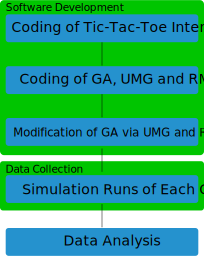
\includegraphics[width=0.5\linewidth]{../figures/procedural_flowchart}
			\caption{Procedural Flowchart}
			\label{fig:proc_flowchart}
		\end{figure}

		The study aims to compare the performance of the genetic algorithms with different elite preservation methods.
		The three are: an unmodified Python implementation of the work of \textcite{bhattSearchNolossStrategies2008}, and two with modified elite preservation methods based on MGs.
		A preliminary for the accomplishment of such task is a game engine for the interaction between trained GA organisms.
		This was coded in Python, as application programming interfaces (APIs) for machine learning have already been implemented in Python.

		After the development of a platform for play of \ttt\ between trained organisms, the development of the required MGs followed.
		The Random Move Generator (RMG) returns one of all possible moves in \ttt\ with equal probability.
		Another MG is Unbeatable Move Generator (UMG).

		UMG is based off of the work of \textcite{barratRobbiebarratUnbeatableTictactoe2019}.
		It is stated to be unbeatable, however, the Move Generator has a small chance of being beat as the second player.
		This makes an ideal opponent for trained organisms, given that the GA will find an exploit eventually.
		In line with this, the GA might be able to use said exploit to have better performance.

		The organisms to be trained were implemented in Python as well.
		The GA was composed of unique genomes with genes for each possible game state with alleles that correspond to the moves to be taken.
		Following the flow represented in Figure~\ref{fig:genetic}, the operators are adapted from \textcite{bhattSearchNolossStrategies2008}.
		The only aspect of the GA that differs from the implementation of that in \textcite{bhattSearchNolossStrategies2008} is the organism representation.

		\subsection{Organism Representation}
			Organisms are represented with genomes, as shown in Figure~\ref{fig:genome}.
			Each gene in the genome represents a game state that considers rotation and symmetry using an implementation of the game-base used by \textcite{bhattSearchNolossStrategies2008}.
			These genes have a corresponding allele that represents the move the organism will take.
			\begin{figure}[htbp]
				\centering
				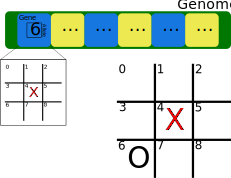
\includegraphics[width=0.75\linewidth]{../figures/representation}
				\caption{Genome of an organism}
				\label{fig:genome}
			\end{figure}

		\subsection{Initial Population}
			For each game state represented by genes in the genome, the organism is given a random possible move for that game state.
			Any valid move in a given game state is considered in choosing the allele randomly.

		\subsection{Selection Operator}
			The following niched fitness equation \autocite{bhattSearchNolossStrategies2008} was used to modify the implementation of the Stochastic Universal Selection operator by \textcite{panchapakesanStochasticUniversalSampling2014}:
			\begin{equation*}
				f_\mathrm{niched}(x_i) = \frac{1}{m} * [1 - f(x_i)]
			\end{equation*}
			where $m$ is the number of organisms with the same fitness.
			Using $\frac{1}{m}$ as a factor produces a niching effect \autocite{bhattSearchNolossStrategies2008}.
			The $[1 - f(x_i)]$ quantity produces the opposite pattern compared to Equation~\ref{eqn:fitness}, where instead of zero as the perfect fitness and one as the worst fitness, zero is the worst fitness and one is the perfect fitness.
			This was done due to the fact that SUS is inherently maximizing \autocite{bhattSearchNolossStrategies2008}.
			In this study, half of the population is selected via SUS.

		\subsection{Crossover Operator}
			Similar to that of \textcite{bhattSearchNolossStrategies2008}, 50 cross-sites are randomly chosen per parent pair which is used to take alternate series of alleles from each parent.
			This produces two new offspring with alleles from each parent.
			The mating pool is linear, with parent pairs formed from a mating pool individual and the individual adjacent to it.
			If the individual is last in the linear mating pool, it is paired with the first individual in the mating pool.

		\subsection{Mutation Operator}
			Using random reset mutation, $n_m$ genes are mutated based on the best fitness in the population.
			This basis is formalized by \textcite{bhattSearchNolossStrategies2008} in the following equation:
			\begin{equation*}
				n_m = 250 * f_\mathrm{minimum} + 10
			\end{equation*}

		\subsection{Controlled Elite Preservation}
			In the control genetic algorithm, the organisms from the population before crossover, the population before mutation, and the population after mutation are sorted by fitness in increasing order.
			The solutions with sorted index $j - 1$ are chosen:
			\begin{equation*}
				j(i) = i + 2N * \frac{(i - 1)(i - 2)}{(N - 1)(N - 2)},~~i = 1, 2, \dots, N
			\end{equation*}

		\subsection{Modified Controlled Elite Preservation}
			The following modifications were made to the elite preservation method to produce two other GAs:
			In UMG-Controlled Elite Preservation, the organisms are sorted by the number of losses of each organism when played against the UMG for 300 games.
			In RMG-Controlled Elite Preservation, the organisms are sorted by the number of losses of each organism when played against the RMG for 300 games.

			In the beginning of the GA the organisms were behaving randomly.
			The fitness function for the organisms was based on the possible results based on an unpredictable opponent, thus every possible win, loss and draw is computed and plugged into Equation~\ref{eqn:fitness} to retrieve the fitness of an organism.
			Through natural selection the \enquote{best} organism prevails.
			When the \enquote{best} organism has zero fitness, the GA stops and snapshots the population for the last time.
			If no zero-fitness organism is found before 500 generations have passed, the GA stops itself.
			Using this method, 30 simulations per elite preservation method was run, with 100 organisms per population.
			The number of generations before a simulation encounters a zero-fitness (based on Equation~\ref{eqn:fitness}) or no-loss solution is recorded for each simulation.

			\begin{align*}
				H_0 & : \mu_\mathrm{UMG} = \mu_\mathrm{fitness} = \mu_\mathrm{RMG} \\
				H_a & : \text{The means are not all equal}
			\end{align*}

			The data was analyzed through the $R$ with the use of Analysis of Variance (ANOVA) which gives the $p$-value to test the hypotheses at a given confidence interval.
			The study utilizes $\alpha = 0.10$.
			Should the alternative hypothesis be true, Tukey Honest Significant Differences (Tukey HSD) is applied to locate the different mean.

	\section{Results}
		% TODO: Results
		\begin{figure}[htbp]
			\centering
			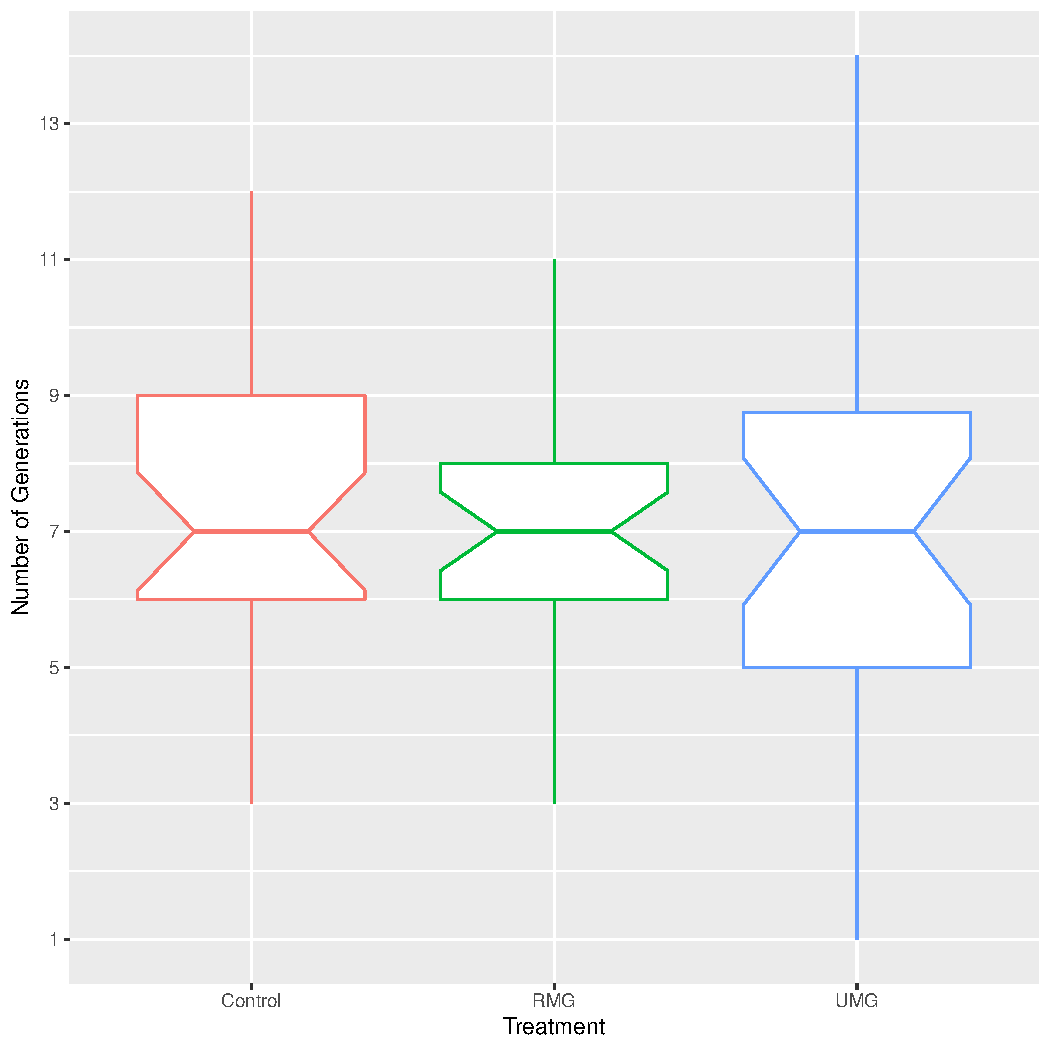
\includegraphics[width=\linewidth]{../figures/boxplot}
			\caption{Notched box plot of treatments}
			\label{fig:boxplot}
		\end{figure}

		A notched box plot of treatment results is shown in Figure~\ref{fig:boxplot}.
		This box plot denotes the interquartile range (IQR) where 50\% of the data is located.
		It is shown that each treatment has a median of seven (7) generations before termination, and the population median is shown by the notches to be within six to eight generations.
		The UMG-controlled GA shows a larger spread while the RMG-controlled GA shows more consistent data points.

		\begin{figure}[htbp]
			\centering
			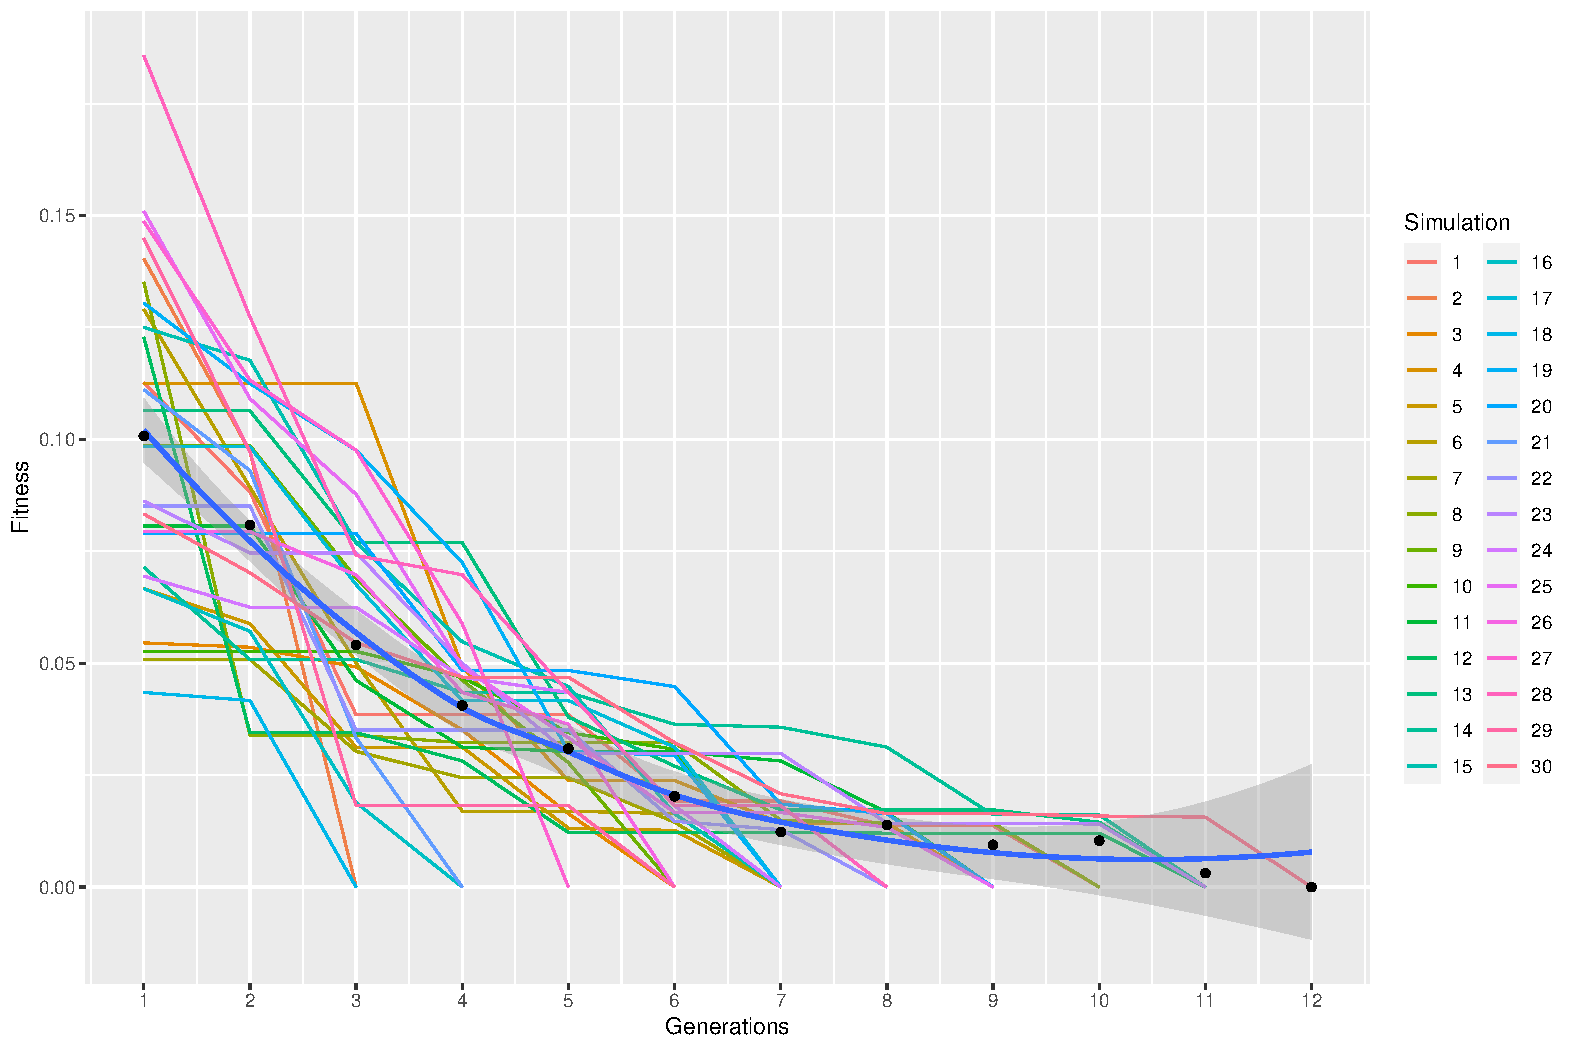
\includegraphics[width=\linewidth]{../figures/ctrl_ftrack}
			\caption{Population-best fitness graph of control}
			\label{fig:fitgraph_ctrl}
		\end{figure}

		The large spread in the data points of the UMG-controlled GA is also evident in Figure~\ref{fig:fitgraph_umg}.
		It is easily shown by the wide standard error bar depicted along the smoothed regression model compared to the standard error bars depicted in Figure~\ref{fig:fitgraph_ctrl} and Figure~\ref{fig:fitgraph_rmg}.
		Figure~\ref{fig:fitgraph_umg} also depicts unique cases where population-best fitness suddenly increases by a large margin.

		This evident spread might invalidate the ANOVA test, thus Bartlett's Test for Homogeneity of Variances was applied to the data via $R$ \autocite{nist/sematechBartlettTest2013}.
		This test resulted in $\chi^2 = 5.1019,~df = 2$ with a $p$-value of 0.07801.
		Said $p$-value is greater than $\alpha = 0.05$, thus the assumption of homogeneity of variances that is necessary in ANOVA is maintained.

		ANOVA was then used to test the null hypothesis that the means of the treatments are equal.
		This returned an F-value of 0.264 and a $p$-value of 0.768.
		The $p$-value is greater than $\alpha = 0.05$, therefore the null hypothesis that the means of the treatments are equal is not rejected.

		\begin{figure}[htbp]
			\centering
			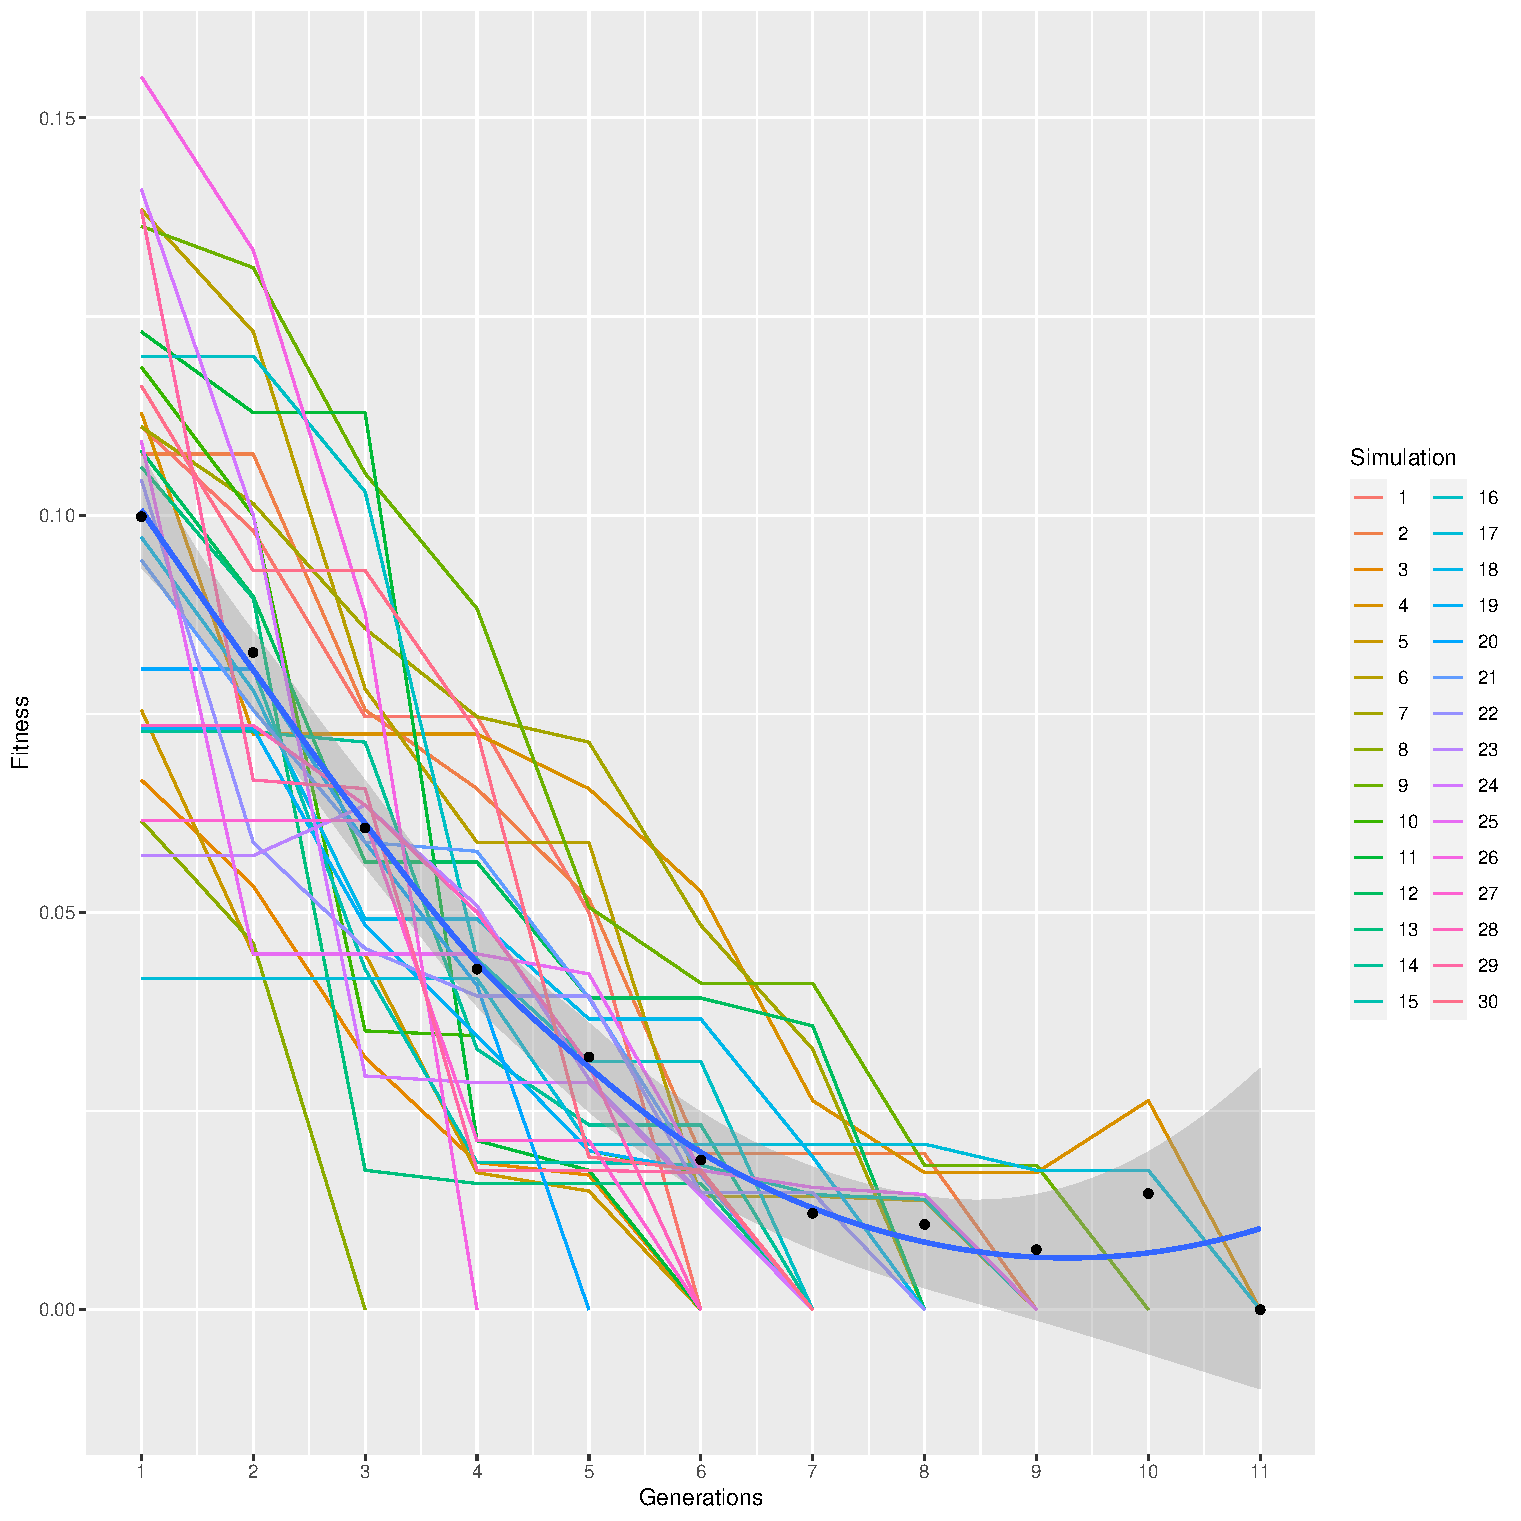
\includegraphics[width=\linewidth]{../figures/rmg_ftrack}
			\caption{Population-best fitness graph of RMG-controlled}
			\label{fig:fitgraph_rmg}
		\end{figure}
		\begin{figure}[htbp]
			\centering
			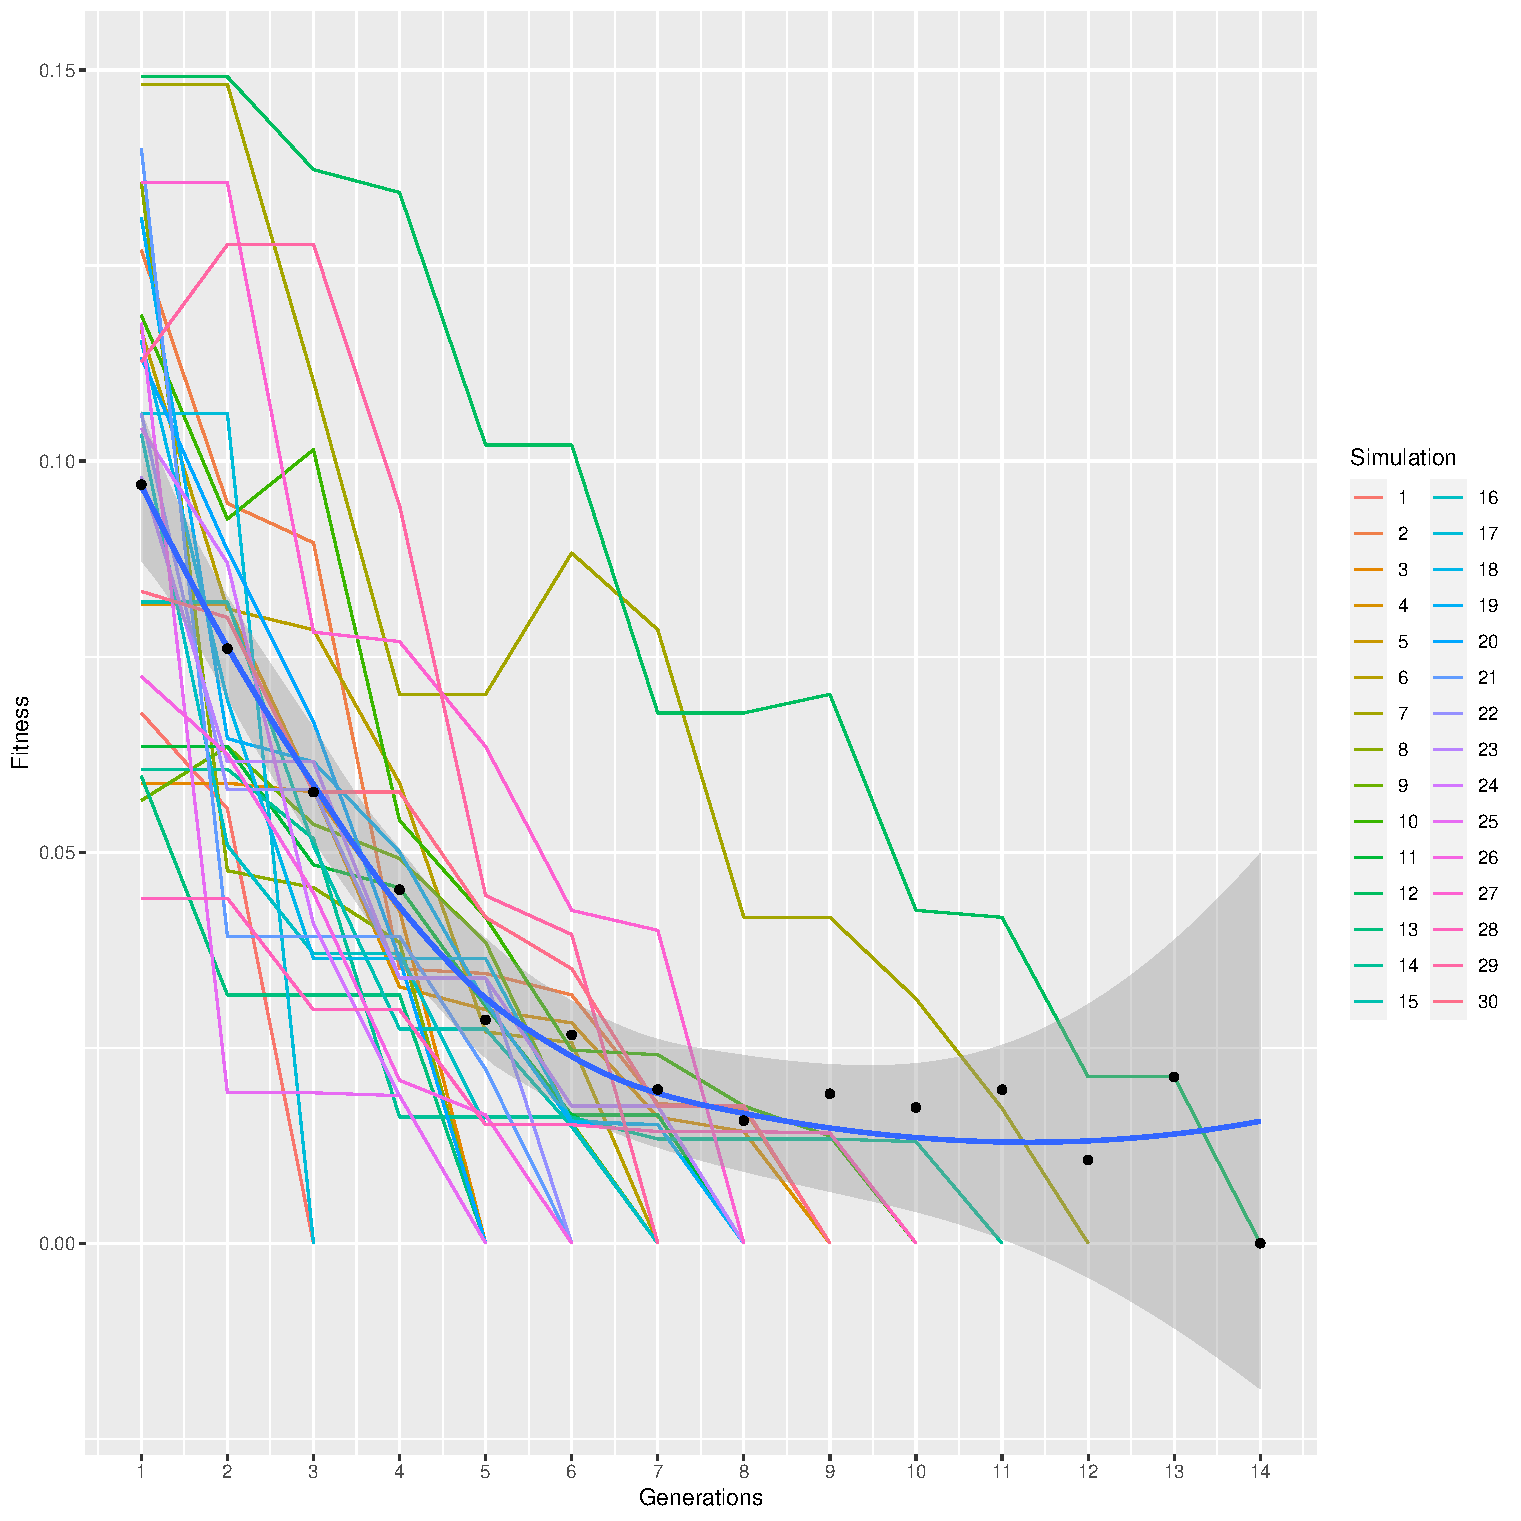
\includegraphics[width=\linewidth]{../figures/umg_ftrack}
			\caption{Population-best fitness graph of UMG-controlled}
			\label{fig:fitgraph_umg}
		\end{figure}

		It can be noted in Figures~\ref{fig:fitgraph_ctrl}, \ref{fig:fitgraph_rmg}, and \ref{fig:fitgraph_umg} that the GAs stop on or before 15 generations.
		This is because the GAs can find no-loss solutions before even surpassing the 500 generation mark.
		The 10-generation worst case tabulated by \textcite{bhattSearchNolossStrategies2008} agrees with these findings.
		The results for each GA are comparatively lower than the 500-generation upper bound used by \textcite{bhattSearchNolossStrategies2008}.
		This can be explained by the fact that the first player is more likely to win in \ttt\ \autocite{cranenburghTicTacToe2007}, thus the game is inherently biased towards the first player.

		The ANOVA test results assert that the modifications have no effect on the number of generations a GA requires to find a no-loss solution.
		This means that the application of an unbeatable opponent did not promote the genetic evolution of the GA towards a no-loss solution.
		This can imply that either the modification was made in a less-effective component, or the application did not change any behaviour of the GA at all.
		The latter implication can be disproven by the discrepancies produced by the UMG-controlled GA demonstrated in Figure~\ref{fig:fitgraph_umg}.
		This behaviour shows that in some cases, the alignments of the UMG goes against the alignments of the fitness function.
		Such behaviour demonstrates that the UMG modification does in fact, affect the evolution of the GA in no small way.

		In the case that the UMG modification was placed in a less-effective component of the GA, it could be implied that there is no effective component in the GA that can accommodate the modification, or that there is one that is not specifically in the Controlled Elite Preservation operator.
		To prove whether there is an effective component in the GA that can utilize the \enquote{unbeatability} of the UMG or not requires extensive research far beyond the scope of this study.

		Either way, this study shows that modifying the Controlled Elite Preservation operator of the GA does not significantly improve the performance of the GA.
		An observation that might be of use, however, is the fact that the UMG-controlled GA shows promise of increase in variability of the GA, which can be used in finding more diverse solutions in the search space.

	\section{Summary and Conclusion}
		% TODO: Summary and Conclusion
		In essence, the stated objectives: to train organisms with MGs and to compare their performance, has been achieved through the modifications to the Controlled Elite Preservation operator.
		This study targeted the Controlled Elite Preservation operator specifically, thus further research is required to acquire more comprehensive data regarding the effects of having a \enquote{smart} opponent control the evolution of a GA.

		The study resulted in proof that modifying the Controlled Elite Preservation operator does not improve the performance of the GA.
		This opens up more questions, on whether or not the application of MG will ever affect the behaviour of a GA.
		It is also recommended to involve testing the performance of the GA as a second player.
		Furthermore, this research serves as a foundation for more extensive investigations into the effects of \enquote{smart} AI on the learning of other AI.

	\section{Acknowledgement}
		% TODO: Acknowledgement
		We are grateful for our friends and family for their continued support in our continuous lives.
		We are also thankful to our teachers, research teacher, and research adviser for their unwavering assistance in having the research completed.
		Without these people, this research would never be successful.

	\printbibliography
\end{document}
